\section*{Bài tập 01}

\subsection*{Phần 1. Tổng quan về máy học}

\paragraph{Câu 1.1}

\textbf{(a) Phân loại và gom cụm.} Phân loại (classification) là bài toán \emph{có giám sát}: tập huấn có nhãn đúng; mô hình học hàm từ đặc trưng sang nhãn rời rạc. Ví dụ: dự đoán email là spam hay không từ nội dung. Gom cụm (clustering) là \emph{không giám sát}: không có nhãn sẵn; thuật toán nhóm các điểm tương tự nhau. Ví dụ: phân khách hàng thành vài nhóm mua sắm dựa trên hành vi, chưa biết trước tên nhóm.

\textbf{(b) Bốn thang đo Stevens — ví dụ thực tế.}
\begin{enumerate}
  \item \emph{Định danh} (nominal): chỉ phân loại, không có thứ tự. Ví dụ: mã màu mắt (nâu, xanh\dots).
  \item \emph{Thứ tự} (ordinal): thứ tự có nghĩa, khoảng cách số chưa chắc đồng nghĩa. Ví dụ: mức độ hài lòng (kém --- trung bình --- tốt).
  \item \emph{Khoảng} (interval): thứ tự và \emph{chênh lệch} có nghĩa; tỷ số giữa hai giá trị thường không có nghĩa; không có ``không'' tuyệt đối theo nghĩa vật lý. Ví dụ: nhiệt độ độ C (0\textdegree{}C không phải ``không nhiệt'').
  \item \emph{Tỷ lệ} (ratio): có điểm không tuyệt đối, tỷ số có nghĩa. Ví dụ: thu nhập (0 nghĩa là không có thu nhập), khối lượng.
\end{enumerate}

\textbf{(c) Quy trình CRISP-DM (các bước chính).}
\begin{enumerate}
  \item \emph{Hiểu nghiệp vụ:} xác định mục tiêu, tiêu chí thành công, ràng buộc.
  \item \emph{Hiểu dữ liệu:} thu thập, khám phá sơ bộ, chất lượng ban đầu.
  \item \emph{Chuẩn bị dữ liệu:} làm sạch, tích hợp, biến đổi, rời rạc hóa nếu cần.
  \item \emph{Mô hình hóa:} chọn kỹ thuật, huấn luyện, điều chỉnh tham số.
  \item \emph{Đánh giá:} kiểm tra đủ tốt với mục tiêu nghiệp vụ, không chỉ độ chính xác kỹ thuật.
  \item \emph{Triển khai:} đưa vào vận hành, giám sát và cập nhật chu trình nếu dữ liệu hoặc nghiệp vụ thay đổi.
\end{enumerate}

\textbf{(d) Phân loại và hồi quy.} Phân loại: đầu ra là nhãn lớp rời rạc. Ví dụ: chẩn đoán có/không bệnh. Hồi quy: đầu ra là biến liên tục (hoặc số thực). Ví dụ: dự báo giá nhà từ diện tích và vị trí.

\textbf{(e) Chất lượng dữ liệu và xử lý thường gặp.}
\begin{itemize}
  \item \emph{Nhiễu:} sai lệch ngẫu nhiên --- làm mịn, lọc, hoặc thu thập lại.
  \item \emph{Giá trị ngoại lai (outliers):} điểm bất thường --- kiểm tra lỗi nhập, cắt/winsorize, hoặc mô hình chịu ngoại lai.
  \item \emph{Thiếu giá trị:} điền (mean/median/mode), mô hình hỗ trợ thiếu, hoặc loại bỏ có kiểm soát.
  \item \emph{Trùng lặp:} gộp hoặc xóa bản ghi trùng để tránh lệch trọng số.
\end{itemize}

\textbf{(f) Rò rỉ dữ liệu (data leakage).} Là khi thông tin từ ``tương lai'' hoặc từ nhãn lọt vào đặc trưng huấn luyện, làm đánh giá quá lạc quan và mô hình kém khi áp dụng thật. Nguy hiểm vì ta tưởng mô hình tốt nhưng trên dữ liệu mới sẽ sai. Ví dụ: dùng cột ``tổng chi phương điều trị'' để dự đoán ``có nhập viện hay không'' khi cột đó chỉ có sau khi điều trị --- đã mang thông tin kết quả.

\subsection*{Phần 2. Phân tích khám phá và tiền xử lý}

\subsubsection*{Câu 2.1}

Dãy tuổi đã sắp tăng ($n=27$):
\begin{center}
\small
$\begin{aligned}
&13,15,16,16,19,20,20,21,22,22,25,25,25,25,30,33,33,\\
&35,35,35,35,36,40,45,46,52,70.
\end{aligned}$
\end{center}

\textbf{(a) Trung bình, trung vị, mốt.}

Tổng các giá trị bằng $809$, nên trung bình mẫu
\[
\bar x=\frac{809}{27}\approx 29{,}96.
\]

Vì $n$ lẻ, trung vị là phần tử vị trí thứ $\frac{n+1}{2}=14$ trên dãy đã sắp, đó là $25$.

Đếm tần số: $25$ và $35$ mỗi giá trị xuất hiện $4$ lần; các giá trị khác không quá $2$ lần. Vậy có hai mốt: $25$ và $35$ (đa mốt).

\textbf{(b) Tứ phân vị $Q_1$, $Q_3$.}

Có hai quy ước phổ biến; đề cho phép xấp xỉ.

\emph{Cách vị trí nguyên (1-based):} $Q_1$ ứng vị trí $\frac{1}{4}(n+1)=7$ $\Rightarrow$ giá trị thứ $7$ là $20$. $Q_3$ ứng vị trí $\frac{3}{4}(n+1)=21$ $\Rightarrow$ giá trị thứ $21$ là $35$. Khi đó $\mathrm{IQR}=35-20=15$.

\emph{Cách nội suy tuyến tính giữa hai quan sát kề:} vị trí $Q_1$ là $7{,}5$ nên $Q_1=\frac{20+21}{2}=20{,}5$; vị trí $Q_3$ là $20{,}5$ nên $Q_3=\frac{35+35}{2}=35$ và $\mathrm{IQR}=14{,}5$.

\textbf{(c) Boxplot và nhận xét.}

Năm số tóm tắt: $\min=13$, trung vị $=25$, $\max=70$; $Q_1,Q_3$ chọn một trong hai cách trên (minh họa: $Q_1=20{,}5$, $Q_3=35$ nếu nội suy). Với $\mathrm{IQR}=14{,}5$, ngưỡng trên Tukey $Q_3+1{,}5\cdot\mathrm{IQR}=56{,}75$; vì $70>56{,}75$ nên $70$ thường được xem là ngoại lai phía trên. Trung bình ($\approx29{,}96$) lớn hơn trung vị ($25$) --- phân bố \emph{lệch phải} (đuôi dài về giá trị lớn).

\begin{center}
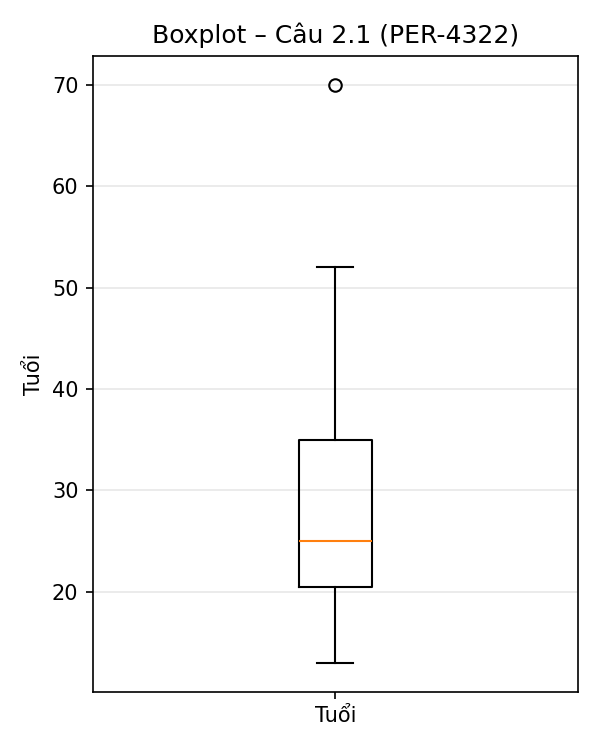
\includegraphics[width=0.55\textwidth]{boxplot_tuoi_cau2_1.png}
\end{center}
\textit{Hình:} boxplot thuộc tính tuổi (cùng dữ liệu đề; râu và điểm ngoại lai theo quy ước $1{,}5\cdot\mathrm{IQR}$ thông dụng).

\textbf{(d) Rời rạc hóa $k=4$.}

\emph{Chia độ rộng đều:} $\min=13$, $\max=70$, bước $w=\frac{70-13}{4}=14{,}25$. Các khoảng (ý niệm các nửa khoảng có thể ghi theo quy ước lớp):
\[
(13;\,27{,}25],\quad (27{,}25;\,41{,}5],\quad (41{,}5;\,55{,}75],\quad (55{,}75;\,70].
\]
Số mẫu từng khoảng: $14$, $9$, $3$, $1$ (tổng $27$).

\emph{Chia gần tần số đều:} chia $27$ mẫu thành $7+7+7+6$ theo thứ tự đã sắp: nhóm 1 --- $13$ đến $20$; nhóm 2 --- $21$ đến $25$; nhóm 3 --- $30$ đến $35$; nhóm 4 --- $36$ đến $70$.

\subsubsection*{Câu 2.2}

\textbf{Bước 1 --- Thang đo của $V$.} Các giá trị $1,\ldots,5$ có thứ tự và khoảng cách giữa hai mức liền kề đều bằng $1$, nên hiệu có ý nghĩa; không có ``số không'' tuyệt đối theo nghĩa tỷ lệ vật lý, và tỷ số $2/1$ chưa hẳn mang nghĩa ``gấp đôi khối lượng''. Vì vậy $V$ phù hợp \emph{thang khoảng} (interval), hơn là thuần định danh/thứ tự, và không cần là thang tỷ lệ.

\textbf{Bước 2 --- Cùng thang khoảng với $V$.} Hai biểu diễn cùng thang khoảng nếu tồn tại $a>0$, $b$ sao cho $W=aV+b$ đúng trên cả năm mức $V\in\{1,\ldots,5\}$.

\begin{itemize}
  \item $W_1=100V$ (lấy $a=100$, $b=0$) --- \emph{cùng thang khoảng.}
  \item $W_2=V+9$ --- \emph{cùng.}
  \item $W_3$: dãy $8,13,45,6,7$ không tăng dần cùng $V$, không tồn tại $a,b$ để $W=aV+b$ --- \emph{không cùng.}
  \item $W_4=V^2$: các bước $W(2)-W(1)=3$, $W(3)-W(2)=5$ khác nhau --- không tuyến tính theo $V$ --- \emph{không cùng thang khoảng.}
  \item $W_5=2V-12$ --- \emph{cùng.}
  \item $W_6=3V$ --- \emph{cùng.}
\end{itemize}

\medskip
\textit{Kết luận:} Cùng thang khoảng với $V$: $W_1,W_2,W_5,W_6$. Không: $W_3,W_4$.

\subsection*{Phần 3. Huấn luyện và đánh giá}

\subsubsection*{Câu 3.1}

Nhãn thực $ABCABCABCA$, nhãn dự đoán $ACCBBAABCC$ ($n=10$).

Duyệt từng mẫu và đếm (hàng $=$ thực, cột $=$ dự):

\begin{center}
\begin{tabular}{c|ccc}
      & dự $A$ & dự $B$ & dự $C$ \\\hline
thực $A$ & $2$ & $1$ & $1$ \\
thực $B$ & $0$ & $2$ & $1$ \\
thực $C$ & $1$ & $0$ & $2$ \\
\end{tabular}
\end{center}

Số đúng trên đường chéo: $2+2+2=6$.

\[
\text{Accuracy}=\frac{6}{10}=0{,}6.
\]

Với mỗi lớp $k$: $\mathrm{TP}_k$ là ô $(k,k)$, $\mathrm{FN}_k$ là tổng hàng trừ $\mathrm{TP}_k$, $\mathrm{FP}_k$ là tổng cột trừ $\mathrm{TP}_k$;
\[
P_k=\frac{\mathrm{TP}_k}{\mathrm{TP}_k+\mathrm{FP}_k},\quad
R_k=\frac{\mathrm{TP}_k}{\mathrm{TP}_k+\mathrm{FN}_k},\quad
F1_k=\frac{2P_kR_k}{P_k+R_k}.
\]

\begin{itemize}
  \item Lớp $A$: $\mathrm{TP}=2$, $\mathrm{FP}=1$, $\mathrm{FN}=2$ $\Rightarrow$ $P=\frac{2}{3}$, $R=\frac{1}{2}$, $F1\approx0{,}571$.
  \item Lớp $B$: $\mathrm{TP}=2$, $\mathrm{FP}=1$, $\mathrm{FN}=1$ $\Rightarrow$ $P=R=\frac{2}{3}$, $F1\approx0{,}667$.
  \item Lớp $C$: $\mathrm{TP}=2$, $\mathrm{FP}=2$, $\mathrm{FN}=1$ $\Rightarrow$ $P=0{,}5$, $R=\frac{2}{3}$, $F1\approx0{,}571$.
\end{itemize}

\subsubsection*{Câu 3.2 (hồ sơ 14 mẫu và danh sách quy tắc)}

Quy tắc theo thứ tự: (1) nếu thuộc tính \emph{outlook} là \emph{overcast} thì \emph{play} là \emph{yes}; (2) nếu không thỏa (1) và \emph{windy} là đúng thì \emph{play} là \emph{no}; (3) nếu không thỏa (1)--(2) và \emph{outlook} là \emph{sunny} thì \emph{no}; (4) còn lại thì \emph{yes}.

Áp dụng từng dòng (tóm tắt kết quả dự đoán so với thực tế):

\begin{center}
\small
\begin{tabular}{rllllcc}
STT & outlook & windy & dự đoán & thực & đúng?\\\hline
1 & sunny & F & no & no & OK \\
2 & sunny & T & no & no & OK \\
3 & overcast & F & yes & yes & OK \\
4 & rainy & F & yes & yes & OK \\
5 & rainy & F & yes & yes & OK \\
6 & rainy & T & no & no & OK \\
7 & overcast & T & yes & yes & OK \\
8 & sunny & F & no & no & OK \\
9 & sunny & F & no & yes & Sai \\
10 & rainy & F & yes & yes & OK \\
11 & sunny & T & no & yes & Sai \\
12 & overcast & T & yes & yes & OK \\
13 & overcast & F & yes & yes & OK \\
14 & rainy & T & no & no & OK \\
\end{tabular}
\end{center}

Lớp dương: nhãn \emph{play} là \emph{yes}. Ma trận nhầm lẫn $2\times 2$ (hàng $=$ thực, cột $=$ dự):

\begin{center}
\begin{tabular}{c|cc}
      & dự yes & dự no \\\hline
thực yes & $7$ & $2$ \\
thực no  & $0$ & $5$ \\
\end{tabular}
\end{center}

$\mathrm{TP}=7$, $\mathrm{FN}=2$, $\mathrm{FP}=0$, $\mathrm{TN}=5$, $N=14$.

\[
\text{Accuracy}=\frac{12}{14}=\frac{6}{7}\approx0{,}857,\quad
P=\frac{7}{7}=1,\quad
R=\frac{7}{9}=\frac{7}{9}\approx0{,}778,
\]
\[
\text{Specificity}=\frac{5}{5}=1,\quad
F1=\frac{2PR}{P+R}=\frac{7}{8}=0{,}875.
\]
